\documentclass[12pt,a4paper]{article}

\usepackage{amsmath,amssymb,amsthm}
\usepackage{mathtools}
\usepackage{tikz}
\usetikzlibrary{arrows.meta,positioning,cd}
\usepackage{enumitem}
\usepackage[margin=2.5cm]{geometry}
\usepackage{hyperref}
\usepackage{booktabs}

% Theorem environments
\newtheorem{theorem}{Theorem}[section]
\newtheorem{proposition}[theorem]{Proposition}
\newtheorem{lemma}[theorem]{Lemma}
\newtheorem{corollary}[theorem]{Corollary}
\theoremstyle{definition}
\newtheorem{definition}[theorem]{Definition}
\newtheorem{example}[theorem]{Example}
\theoremstyle{remark}
\newtheorem{remark}[theorem]{Remark}

% Shortcuts
\newcommand{\C}{\mathbb{C}}
\newcommand{\Z}{\mathbb{Z}}
\newcommand{\N}{\mathbb{N}}
\newcommand{\F}{\mathbb{F}}
\newcommand{\End}{\operatorname{End}}
\newcommand{\Hom}{\operatorname{Hom}}
\newcommand{\Ind}{\operatorname{Ind}}
\newcommand{\Res}{\operatorname{Res}}
\newcommand{\id}{\mathrm{id}}
\newcommand{\im}{\operatorname{im}}
\newcommand{\coker}{\operatorname{coker}}
\newcommand{\Rep}{\mathcal{R}\mathrm{ep}}
\newcommand{\Vect}{\mathcal{V}\!\mathit{ect}}
\newcommand{\GL}{\mathrm{GL}}
\newcommand{\op}{\mathrm{op}}
\newcommand{\Set}{\mathcal{S}\!\mathit{et}}

\title{Limits and Colimits in $\Rep(G)$}
\author{Notes}
\date{}

\begin{document}
\maketitle

\begin{abstract}
We explore a number of natural examples of limits and colimits in the category
of representations of a finite group~$G$. We shall see that limits correspond to
sub-representations and colimits correspond to quotient representations. We
carefully distinguish these from the Hopf algebra multiplication and
comultiplication on the group algebra $\C G$.
\end{abstract}

\tableofcontents

%% =================================================================
\section{Setup}
%% =================================================================

Let $G$ be a fixed finite group (for example $S_n$ or $\GL_n(\F_q)$).
A \emph{representation} of $G$ is a finite-dimensional complex vector space $V$
together with a group homomorphism $\rho\colon G \to \GL(V)$. A morphism of representations $\varphi\colon V \to W$
is a $\C$-linear map satisfying $\varphi(g \cdot v) = g \cdot \varphi(v)$ for all
$g \in G$, $v \in V$ (equivariance).
Write $\Rep(G)$ for the category of finite-dimensional complex representations of~$G$.

%% =================================================================
\section{Limits and colimits}
%% =================================================================

Start with some representations and some equivariant maps between them ---
call this a \emph{diagram}.

\begin{definition}
The \textbf{limit} of a diagram is the \emph{most general representation that maps
into every object in the diagram, compatibly with all the maps}. ``Most general''
means: any other representation that maps in compatibly must factor through it uniquely.

The \textbf{colimit} is the dual: the \emph{most general representation that every
object in the diagram maps into}, compatibly.
\end{definition}

The simplest diagram is two representations with no maps between them: just
$V$ and $W$ sitting side by side. The limit and colimit of this diagram are the
\textbf{product} and \textbf{coproduct}.

The \textbf{product} $V \times W$ is the limit: the most general representation
that maps into both $V$ and $W$. It comes with projections $\pi_1\colon V \times W \to V$
and $\pi_2\colon V \times W \to W$, and its universal property says: for any $X$ with
equivariant maps $f\colon X \to V$ and $g\colon X \to W$, there is a unique
$h\colon X \to V \times W$ with $\pi_1 \circ h = f$ and $\pi_2 \circ h = g$.
\[
\begin{tikzcd}[row sep=large, column sep=large]
& X \arrow[dl, "f"'] \arrow[d, dashed, "\exists! \, h" description] \arrow[dr, "g"] & \\
V & V \times W \arrow[l, "\pi_1"] \arrow[r, "\pi_2"'] & W
\end{tikzcd}
\]
The arrows go \emph{out} of $V \times W$. The universal property says $V \times W$ is
the ``best'' representation that maps out to both $V$ and $W$.

The \textbf{coproduct} $V \sqcup W$ is the colimit: the most general representation
that both $V$ and $W$ map into. It comes with inclusions $\iota_1\colon V \to V \sqcup W$
and $\iota_2\colon W \to V \sqcup W$, and its universal property says: for any $X$ with
equivariant maps $f\colon V \to X$ and $g\colon W \to X$, there is a unique
$h\colon V \sqcup W \to X$ with $h \circ \iota_1 = f$ and $h \circ \iota_2 = g$.
\[
\begin{tikzcd}[row sep=large, column sep=large]
V \arrow[r, "\iota_1"] \arrow[dr, "f"'] & V \sqcup W \arrow[d, dashed, "\exists! \, h" description]
  & W \arrow[l, "\iota_2"'] \arrow[dl, "g"] \\
& X &
\end{tikzcd}
\]
The arrows go \emph{into} $V \sqcup W$. The universal property says $V \sqcup W$ is
the ``best'' representation that both $V$ and $W$ map into.

\medskip

In $\Rep(G)$, the product turns out to equal the coproduct, every limit is a
\textbf{sub-representation}, and every colimit is a \textbf{quotient representation}.
The object that is simultaneously the product and coproduct is the biproduct
$V \oplus W$. We construct it next.

%% =================================================================
\section{The biproduct}
%% =================================================================

\begin{definition}
Given representations $V$ and $W$, the \emph{biproduct} $V \oplus W$ is:
\begin{itemize}
  \item \textbf{Underlying space:} $\{(v,w) : v \in V,\; w \in W\}$.
  \item \textbf{$G$-action:} $g \cdot (v,w) = (g \cdot v,\; g \cdot w)$.
  \item \textbf{Four structure maps:}
\end{itemize}
\[
\begin{tikzcd}[column sep=large]
V \arrow[r, "\iota_1"] & V \oplus W \arrow[r, "\pi_1"] & V \\
W \arrow[r, "\iota_2"'] & V \oplus W \arrow[r, "\pi_2"'] & W
\end{tikzcd}
\]
where $\iota_1(v) = (v,0)$, $\iota_2(w) = (0,w)$, $\pi_1(v,w) = v$, $\pi_2(v,w) = w$.
\end{definition}

The structure maps satisfy:
\begin{align}
\pi_1 \circ \iota_1 &= \id_V & \pi_1 \circ \iota_2 &= 0 \\
\pi_2 \circ \iota_1 &= 0     & \pi_2 \circ \iota_2 &= \id_W
\end{align}
All four maps are equivariant.

%% =================================================================
\section{From biproduct to product}
%% =================================================================

Forget the inclusions $\iota_1, \iota_2$. Keep only the projections.

The product is the limit of the diagram $V \quad W$ (two objects, no morphisms).
A cone is an object $X$ with maps $X \to V$ and $X \to W$; the universal cone is the
product.

\begin{proposition}
$(V \oplus W, \pi_1, \pi_2)$ is the product of $V$ and $W$ in $\Rep(G)$.
\end{proposition}

\begin{proof}
Given equivariant $f\colon X \to V$ and $g\colon X \to W$, we must find a unique
equivariant $h\colon X \to V \oplus W$ with $\pi_1 \circ h = f$ and
$\pi_2 \circ h = g$.

\medskip
\begin{center}
\begin{tikzcd}[row sep=large, column sep=large]
& X \arrow[dl, "f"'] \arrow[d, dashed, "h" description] \arrow[dr, "g"] & \\
V & V \oplus W \arrow[l, "\pi_1"] \arrow[r, "\pi_2"'] & W
\end{tikzcd}
\end{center}

\textbf{Existence.} Define $h(x) = (f(x), g(x))$. Then $\pi_1 \circ h = f$ and
$\pi_2 \circ h = g$. Equivariance: for any $\gamma \in G$,
$h(\gamma \cdot x) = (f(\gamma \cdot x), g(\gamma \cdot x))
= (\gamma \cdot f(x), \gamma \cdot g(x)) = \gamma \cdot h(x)$.

\textbf{Uniqueness.} If $\pi_1 \circ h' = f$ and $\pi_2 \circ h' = g$, then
\[
h'(x) = (\pi_1(h'(x)),\, \pi_2(h'(x))) = (f(x), g(x)) = h(x). \qedhere
\]
\end{proof}

\begin{remark}
No addition of morphisms was needed. The product universal property only requires
pairing, which is a set-level operation.
\end{remark}

%% =================================================================
\section{From biproduct to coproduct}
%% =================================================================

Forget the projections $\pi_1, \pi_2$. Keep only the inclusions.

The coproduct is the colimit of the same diagram $V \quad W$. A cocone is an object $X$
with maps $V \to X$ and $W \to X$; the universal cocone is the coproduct.

\begin{proposition}
$(V \oplus W, \iota_1, \iota_2)$ is the coproduct of $V$ and $W$ in $\Rep(G)$.
\end{proposition}

\begin{proof}
Given equivariant $f\colon V \to X$ and $g\colon W \to X$, we must find a unique
equivariant $h\colon V \oplus W \to X$ with $h \circ \iota_1 = f$ and
$h \circ \iota_2 = g$.

\medskip
\begin{center}
\begin{tikzcd}[row sep=large, column sep=large]
V \arrow[r, "\iota_1"] \arrow[dr, "f"'] & V \oplus W \arrow[d, dashed, "h" description]
  & W \arrow[l, "\iota_2"'] \arrow[dl, "g"] \\
& X &
\end{tikzcd}
\end{center}

\textbf{Existence.} Define $h(v,w) = f(v) + g(w)$. Then $h \circ \iota_1(v) =
h(v,0) = f(v) + g(0) = f(v)$, and similarly $h \circ \iota_2 = g$. Equivariance
follows from linearity of $f$ and $g$.

\textbf{Uniqueness.} Suppose $h' \circ \iota_1 = f$ and $h' \circ \iota_2 = g$.
Then by linearity of $h'$:
\[
h'(v,w) = h'((v,0) + (0,w)) = h'(\iota_1(v)) + h'(\iota_2(w)) = f(v) + g(w) = h(v,w). \qedhere
\]
\end{proof}

\begin{remark}
This direction requires \textbf{addition}: we use $f(v) + g(w)$ to define $h$, and
linearity of $h'$ to prove uniqueness. This is why the coproduct universal property
needs the additive structure of $\Vect$, while the product does not.
\end{remark}

%% =================================================================
\section{Limits: subspaces}
%% =================================================================

\subsection{Kernel}

Given equivariant $f\colon V \to W$, define
$\ker(f) = \{v \in V : f(v) = 0\}$ with the inherited $G$-action, and let
$\iota\colon \ker(f) \hookrightarrow V$ be the inclusion.

\medskip
\begin{center}
\begin{tikzcd}
\ker(f) \arrow[r, hook, "\iota"] & V \arrow[r, "f"] & W
\end{tikzcd}
\end{center}

First, $\ker(f)$ is a sub-representation: if $v \in \ker(f)$ and $g \in G$, then
$f(g \cdot v) = g \cdot f(v) = g \cdot 0 = 0$, so $g \cdot v \in \ker(f)$.

\begin{proposition}[Kernel is a limit]
$\ker(f)$ satisfies the following universal property: for any equivariant
$\varphi\colon X \to V$ with $f \circ \varphi = 0$, there exists a unique equivariant
$\bar\varphi\colon X \to \ker(f)$ with $\iota \circ \bar\varphi = \varphi$.
\end{proposition}

\begin{center}
\begin{tikzcd}[row sep=large]
X \arrow[dr, "\varphi"] \arrow[d, dashed, "\exists! \, \bar\varphi"'] & \\
\ker(f) \arrow[r, hook, "\iota"'] & V \arrow[r, "f"'] & W
\end{tikzcd}
\end{center}

This is the universal property of a limit: $\ker(f)$ is the most general
representation that maps into $V$ with the constraint that the composite
to $W$ is zero. Any other such representation factors through it uniquely.

\begin{proof}
Since $f \circ \varphi = 0$, we have $\im(\varphi) \subseteq \ker(f)$, so
$\bar\varphi(x) = \varphi(x)$ (viewed in $\ker(f)$) is well-defined and
equivariant. Uniqueness: $\iota$ is injective, so $\iota \circ \bar\varphi
= \varphi$ determines $\bar\varphi$ completely.
\end{proof}

\subsection{Pullback}

The pullback is the limit of the cospan diagram $V \xrightarrow{f} X \xleftarrow{g} W$.
A cone is an object $Y$ with maps $Y \to V$ and $Y \to W$ making the square commute.

Concretely, given equivariant $f\colon V \to X$ and $g\colon W \to X$, the pullback is
\[
V \times_X W = \{(v,w) \in V \oplus W : f(v) = g(w)\}
\]
with the inherited $G$-action.

\medskip
\begin{center}
\begin{tikzcd}[row sep=large, column sep=large]
V \times_X W \arrow[r, "p_2"] \arrow[d, "p_1"']
  \arrow[dr, phantom, "\lrcorner" very near start] & W \arrow[d, "g"] \\
V \arrow[r, "f"'] & X
\end{tikzcd}
\end{center}

This is a subspace of $V \oplus W$ --- precisely, it is the equaliser of
$f \circ \pi_1$ and $g \circ \pi_2\colon V \oplus W \rightrightarrows X$.

%% =================================================================
\section{Colimits: quotients}
%% =================================================================

\subsection{Cokernel}

Given equivariant $f\colon V \to W$, define
$\coker(f) = W / \im(f)$ with the quotient $G$-action $g \cdot [w] = [g \cdot w]$,
and let $q\colon W \twoheadrightarrow \coker(f)$ be the projection.

\medskip
\begin{center}
\begin{tikzcd}
V \arrow[r, "f"] & W \arrow[r, two heads, "q"] & \coker(f)
\end{tikzcd}
\end{center}

First, $\im(f)$ is a sub-representation: if $w = f(v) \in \im(f)$, then
$g \cdot w = g \cdot f(v) = f(g \cdot v) \in \im(f)$. The quotient action is
well-defined: if $w - w' \in \im(f)$, then
$g \cdot w - g \cdot w' = g \cdot (w - w') \in \im(f)$, so $[g \cdot w] = [g \cdot w']$.

\begin{proposition}[Cokernel is a colimit]
$\coker(f)$ satisfies the following universal property: for any equivariant
$\psi\colon W \to X$ with $\psi \circ f = 0$, there exists a unique equivariant
$\bar\psi\colon \coker(f) \to X$ with $\bar\psi \circ q = \psi$.
\end{proposition}

\begin{center}
\begin{tikzcd}[row sep=large]
V \arrow[r, "f"] & W \arrow[r, two heads, "q"] \arrow[dr, "\psi"'] & \coker(f) \arrow[d, dashed, "\exists! \, \bar\psi"] \\
& & X
\end{tikzcd}
\end{center}

This is the universal property of a colimit: $\coker(f)$ is the most general
representation that $W$ maps into with the constraint that the composite from $V$
is zero. Any other such representation receives a unique map from it.

\begin{proof}
Since $\psi \circ f = 0$, we have $\im(f) \subseteq \ker(\psi)$, so
$\bar\psi([w]) = \psi(w)$ is well-defined. Equivariance:
$\bar\psi(g \cdot [w]) = \bar\psi([g \cdot w]) = \psi(g \cdot w) = g \cdot \psi(w)
= g \cdot \bar\psi([w])$.
Uniqueness: $q$ is surjective, so $\bar\psi \circ q = \psi$ determines $\bar\psi$.
\end{proof}

\subsection{Pushout}

The pushout is the colimit of the span diagram $V \xleftarrow{f} X \xrightarrow{g} W$.
A cocone is an object $Y$ with maps $V \to Y$ and $W \to Y$ making the square commute.

Concretely, given equivariant $f\colon X \to V$ and $g\colon X \to W$, the pushout is
\[
V \sqcup_X W = (V \oplus W) / \{(f(x), -g(x)) : x \in X\}
\]
with the quotient $G$-action.

\medskip
\begin{center}
\begin{tikzcd}[row sep=large, column sep=large]
X \arrow[r, "g"] \arrow[d, "f"']
  \arrow[dr, phantom, "\ulcorner" very near end] & W \arrow[d, "j_2"] \\
V \arrow[r, "j_1"'] & V \sqcup_X W
\end{tikzcd}
\end{center}

This is a quotient of $V \oplus W$ --- precisely, it is the coequaliser of
$\iota_1 \circ f$ and $\iota_2 \circ g\colon X \rightrightarrows V \oplus W$.

%% =================================================================
\section{The big picture}
%% =================================================================

Every limit in $\Rep(G)$ is a \textbf{subspace} of something built from the inputs.
Every colimit is a \textbf{quotient} of something built from the inputs. These two
families meet at the biproduct:

\bigskip
\begin{center}
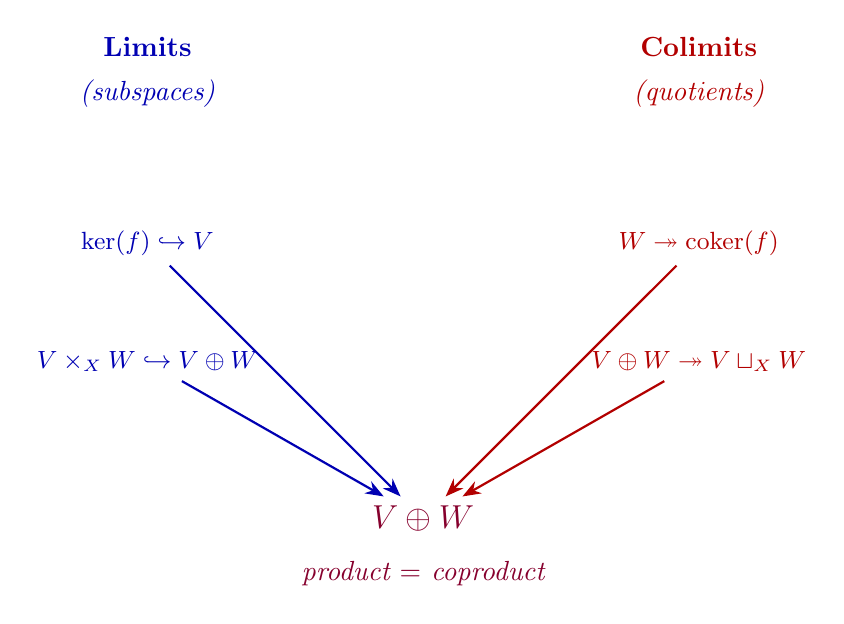
\begin{tikzpicture}[
  every node/.style={font=\small},
  limit/.style={blue!70!black},
  colimit/.style={red!70!black},
  meet/.style={purple!70!black},
  >=Stealth
]
% Left column: limits
\node[limit, font=\bfseries] at (-3.5, 4) {Limits};
\node[limit, font=\itshape] at (-3.5, 3.4) {(subspaces)};

\node[limit] (ker) at (-3.5, 1.5) {$\ker(f) \hookrightarrow V$};
\node[limit] (pb)  at (-3.5, 0) {$V \times_X W \hookrightarrow V \oplus W$};

% Right column: colimits
\node[colimit, font=\bfseries] at (3.5, 4) {Colimits};
\node[colimit, font=\itshape] at (3.5, 3.4) {(quotients)};

\node[colimit] (coker) at (3.5, 1.5) {$W \twoheadrightarrow \coker(f)$};
\node[colimit] (po)    at (3.5, 0) {$V \oplus W \twoheadrightarrow V \sqcup_X W$};

% Center: biproduct
\node[meet, font=\bfseries\large] (bip) at (0, -2) {$V \oplus W$};
\node[meet, font=\itshape] at (0, -2.7) {product $=$ coproduct};

% Arrows converging
\draw[limit, thick, ->] (ker) -- (bip);
\draw[limit, thick, ->] (pb)  -- (bip);
\draw[colimit, thick, ->] (coker) -- (bip);
\draw[colimit, thick, ->] (po)    -- (bip);
\end{tikzpicture}
\end{center}

\bigskip

The pullback is a subspace \emph{of} the biproduct. The pushout is a quotient
\emph{of} the biproduct. So the biproduct is the common ground from which limits
carve out subspaces and colimits form quotients.

%% =================================================================
\section{Warning: the Hopf algebra is a different thing}
%% =================================================================

The group algebra $\C G$ is a Hopf algebra, and this induces additional structure
on the category $\Rep(G)$. The Hopf algebra carries four operations, two of which
are also sometimes called product and coproduct --- a source of confusion.

To distinguish them from the categorical notions of the previous sections, we
shall call them multiplication and comultiplication:
\begin{align*}
\text{multiplication} \quad &\mu\colon \C G \otimes \C G \to \C G, & \mu(g_1 \otimes g_2) &= g_1 g_2, \\
\text{comultiplication} \quad &\Delta\colon \C G \to \C G \otimes \C G, & \Delta(g) &= g \otimes g, \\
\text{unit} \quad &\eta\colon \C \to \C G, & \eta(1) &= e, \\
\text{counit} \quad &\varepsilon\colon \C G \to \C, & \varepsilon(g) &= 1, \\
\text{antipode} \quad &S\colon \C G \to \C G, & S(g) &= g^{-1}.
\end{align*}
These are all linear maps between vector spaces --- they are morphisms in $\Vect$,
not in $\Rep(G)$. The Hopf algebra axioms are equations between these linear maps,
diagrams that commute in $\Vect$. But they \emph{induce} structure on $\Rep(G)$:
\begin{itemize}
\item $\Delta$ gives the \textbf{tensor product}: if $V$ and $W$ are representations,
  then $V \otimes W$ becomes one via $g \cdot (v \otimes w) = gv \otimes gw$.
  The formula $gv \otimes gw$ comes from applying $\Delta(g) = g \otimes g$ to each
  tensor factor.
\item $\varepsilon$ gives the \textbf{unit}: the trivial representation $\C$
  (where $g$ acts as $\varepsilon(g) = 1$) satisfies $\C \otimes V \cong V \cong
  V \otimes \C$.
\item $S$ gives \textbf{duals}: the dual $V^*$ has $G$-action
  $(g \cdot \varphi)(v) = \varphi(S(g) \cdot v) = \varphi(g^{-1} \cdot v)$.
\end{itemize}
So $\Rep(G)$ has two independent structures. The biproduct $\oplus$ and the
limits/colimits of sections~3--8 come from the \emph{abelian} structure.
The tensor product $\otimes$, the trivial representation, and duals come from
the \emph{Hopf algebra} structure on $\C G$. Together these make $\Rep(G)$
into a \emph{monoidal category}.

The theory of monoidal categories is beyond the scope of this document.

\begin{remark}
The limits and colimits of sections~3--8 are all computed by performing the
construction in $\Vect$ --- where the analysis is straightforward --- and then
checking that the $G$-action lifts to the result. This check is the content of
every proof in sections~6--7: the kernel is a sub-representation because
equivariance preserves the defining equation, the cokernel is a quotient
representation because the image is $G$-stable, and so on. In this sense, the
abelian structure of $\Rep(G)$ is inherited from $\Vect$, but each construction
requires verification that $G$ respects it.

The Hopf algebra structure of this section is where $G$ actually enters: the
comultiplication $\Delta(g) = g \otimes g$ depends on $G$, and the monoidal
structure it induces on $\Rep(G)$ has no analogue for bare vector spaces.
\end{remark}

\end{document}
